\addcontentsline{toc}{chapter}{Physical Layer e Sicurezza}
\chapter*{\begin{center}\texttt{6 - Livello Fisico e Sicurezza}\end{center}}
\hrulefill \\
\addcontentsline{toc}{section}{Specifiche Ethernet}
\section*{Specifiche fisiche Ethernet}
\index{Ethernet!specifiche fisiche}
\begin{itemize}
    \item 10BaseT, dove 10 è la banda base, T sta per ``Twisted Pair''.
    \begin{itemize}
        \item trasmissione 10mbps in banda base;
        \item sia coassiale che UTP (la cronologia dei cambiamenti nella tecnologia ha fatto: coassiale thick $>$ coassiale thin $>$ doppino CAT3);
        \item lunghezza max cavo: 100 metri;
        \item connettore RJ45, affidabile ed economico, facile da implementare, al contrario del BNC che unisce i coassiali.
    \end{itemize}
    \item 100BaseT, differisce da 10BaseT in:
    \begin{itemize}
        \item la velocità di trasmissione;
        \item ha 3 tipi possibili di connettore:
        \begin{itemize}
            \item 100Base-T4, doppino 4 coppie;
            \item 100Base-TX, doppino 2 coppie;
            \item 100Base-FX, fibra ottica.
        \end{itemize}      
        \item comunque è retrocompatibile con 10BaseT;
    \end{itemize}
    \item Gigabit Ethernet (802.3Z): fino  1Gbps e non retrocompatibile.
    \item Questi standard Ethernet sono tutti a tecnologia CSMA-CD  
\end{itemize}

\noindent Topologia ad Anello:\index{topologia!ad anello}
\begin{figure} [ht]
    \centering
    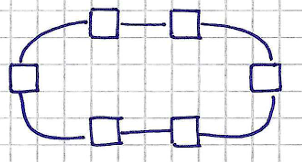
\includegraphics[width=0.5\linewidth]{Figures/06/ringtop.png}
    \caption{Topologia ad anello, supersemplificata.}
    \label{fig:06tknrng}
\end{figure}

\begin{itemize}
    \item semplifica coordinamento accessi;
    \item più facile identificare guasti;
    \item se si guasta un solo elemento, la rete è persa (come i circuiti in serie contrapposti a quelli in parallelo, non so se avete presente il discorso fondamentale dei circuiti elettrici)
\end{itemize}
\noindent Tecnologia ``Token Ring''\index{token ring}: dove il Token è un tipo particolare di frame che dà il permesso agli host per parlare. In Ethernet non c'è modo di stabilire chi può parlare quando. Sul piano Logico, le Token Ring sono disposte ad anello (vedasi Fig. \ref{fig:06tknrng}), ma Fisicamente conviene disporle come stella a doppio anello e utilizzare un MAU, Media/Multistation Access Unit.\\
\noindent Topologia FDDI: Fiber Distributed Data Interface (in disuso),\index{topologia!FDDI} sempre di tipo Token Ring, sempre cablata ad anello o stella, viaggiava a velocità elevate. Usava il doppio anello, due anelli indipendenti (rete autoriparante!).\\

\addcontentsline{toc}{section}{Wireless}
\section*{Livello fisico, reti wireless}
\index{rete, wireless}
\noindent Utilizzano \index{standard!IEEE 802.11}(standard IEEE 802.11\footnote{802.11a : standard per la rete 5 GHz, 802.11b/g : 2.4GHz (802.11b ha max vel. 11Mbps, 802.11g ha max vel. 54Mbps}): \begin{itemize}
    \item radiofrequenze;
    \item infrarossi.
\end{itemize}
\noindent Devono avere un access point\index{access point} collegato alla rete cablata;\\
\noindent L'arbitraggio\index{arbitraggio} del canale trasmissivo si può fare attraverso vari algoritmi (non c'è uno standard preciso);\\
\noindent Velocità di trasmissione: fino a 300Mbps;\\
\noindent Alcune problematiche del caso:\begin{itemize}
    \item propagazione onde radio;
    \item occupazione delle frequenze;
    \item inaffidabilità;
    \item potenza ridotta;
    \item sicurezza.
\end{itemize}
\noindent Più l'host è distante dall'access point, meno sarà la velocità di navigazione (max 50mt circa).\\

\noindent Tipi di interferenze:\index{interferenze}
\begin{itemize}
    \item strutturali: in edifici di cemento armato, la propagazione del segnale è difficile;
    \item su distanze elevate (e.g. ponti radio): edifici, vegetazione, nebbia e fenomeni atmosferici possono disturbare il segnale, le antenne vanno posizionate in un punto adeguato;
    \item dovute ad altre sorgenti: Bluetooth, interfoni per neonati, molti apparecchi utilizzano la frequenza $f = 2.4 GHz$ (con la 5 GHz si verificano meno interferenze).
\end{itemize}

\noindent Modalità di collegamento:
\begin{itemize}
    \item Peer to Peer (P2P): senza passare per l'access point\footnote{Penso che il Peer to Peer in internet sia diverso dal Peer to Peer che si intende qui. Qui penso si intenda una connessione fisica come quella che potremmo fare tra due PC sulla stessa scrivania, magari con tecnologia Bluetooth}. Dipende dalla scheda di rete del dispositivo;
    \item Client - Access Point;
    \item Multiple Access Point \& Roaming. mobilità: l'utente cambia access point mentre si sposta, senza percepire interruzioni di servizio;
    \item Bridging con antenna direzionale
\end{itemize}
\noindent Area di servizio: l'ambito in cui interviene l'access point.\\

\addcontentsline{toc}{subsection}{Sicurezza Wireless}
\subsection*{Sicurezza - Wireless}
\noindent Livelli di sicurezza Wireless:\index{wireless!sicurezza}
\begin{itemize}
    \item open system: detto anche ``con chiave di autenticazione condivisa'', non è esattamente la stessa cosa che dire ``possono entrare tutti''. Vuol dire che è aperta, sì, ma non sono necessariamente la stessa cosa;
    \item WEP: Wired Equivalent Privacy;\index{WEP}
    \item WPA/WPA2: WiFi Protected Access. Queste offrono:\index{WPA/WPA2}
    \begin{itemize}
        \item cifratura dei dati (standard IEEE 802.1X);
        \item integrità dei dati (garanzia che i dati ricevuti sono uguali a quelli spediti, nessuno li ha manomessi lungo il tragitto);
        \item protezione da attacchi Replay\footnote{attacco Replay: catturare pacchetti scambiati tra client e server e replicarli facendoli partire dall'indirizzo dell'attaccante allo scopo di risalire a chiavi di autenticazione.}
    \end{itemize}
\end{itemize}

\noindent WPA:
\begin{itemize}
    \item Personal: privata;
    \item Enterprise: ha bisogno di un Server di Autenticazione (e.g.: Radius, TACACS) che contiene cose come le credenziali degli utenti; 
\end{itemize}

\addcontentsline{toc}{subsection}{Wireless Sensor Network}
\subsection*{Wireless Sensor Network}\index{wireless!sensor network}
\noindent Reti di sensori collegate a controllori come Arduino. I sensori sono dispositivi piccoli, economici, limitati in capacità di elaborazione e trasmissione. Fondamentalmente rilevano delle misurazioni: di luminosità, di temperatura, di umidità, etc.\\
\noindent Caratteristiche delle reti di sensori:
\begin{itemize}
    \item composte da molti sensori che monitorano fenomeni in continuazione;
    \item reti Ad-Hoc, disegnate su misura per ciascuna situazione;
    \item dialogano tra loro tramite antenna;
    \item convergono tutti con i propri dati nel Sink (server centrale);
    \item ZigBee: standard (802.15.4) RL-WPAN, Wireless Personal Area Network; opera su frequenza 2.4 GHz a basso consumo.\index{standard!ZigBee}
\end{itemize}



\begin{wrapfigure}{r}{0.5\textwidth}
 \begin{center}
 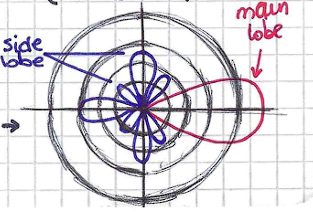
\includegraphics[width=1\linewidth]{Figures/06/onde.png}
    \caption{Diagramma di radiazione supersemplificato}
    \label{fig:06diag}
  \end{center}
\end{wrapfigure}

\noindent Propagazione delle onde:\\
\noindent Potenza di radiazione: la normativa tecnica ETS 300-328 impone di NON irradiare con una potenza EIRP\footnote{Effective Isotropic Radiated Power} $> 100 \text{mW (}\approx 20\text{dBm)}$.\\

\noindent Propagazione:\begin{itemize}
    \item Direzionale: guadagno $>1$;
    \item Omnidirezionale: guadagno $=1$.
\end{itemize}

\noindent Ogni antenna ha il suo diagramma di radiazione per aiutare a capire come orientarla al meglio (sketch in Fig. \ref{fig:06diag}).\\

\noindent Grado di protezione IP\index{IP (Ingress Protection)}(Ingress Protection), indicatore del grado di protezione di un dispositivo da agenti esterni. Formato da 2 cifre:
\begin{itemize}
    \item [I.] (Valore $0\div6$): protezione da oggetti solidi (dove 0 corrisponde a ``nessuna protezione'' e 6 corrisponde a ``protezione totale da polveri'');
    \item [II.] (Valore $0\div8$): permeabilità dell'acqua (dove 0 corrisponde a ``nessuna protezione'' e 8 corrisponde a ``resistente a immersione continua'')
\end{itemize}

\addcontentsline{toc}{section}{Altre specifiche dello Standard 802.3}
\section*{Altre specifiche dello Standard 802.3}\index{standard!IEEE 802.3}
\noindent Ovvero, altro cablaggio.\\

\addcontentsline{toc}{subsection}{Coassiali e Doppini Intrecciati}
\subsection*{Coassiale e Doppino Intrecciato}\index{cavo coassiale}
\begin{itemize}
    \item 10Base5: definisce il cosiddetto ``coassiale thick'' (lunghezza fino a 500m)
    \begin{itemize}
        \item ``thicknet'':\index{cavo coassiale!thicknet} consisteva in un unico bus coassiale, ciascuna macchina per collegarsi al bus aveva bisogno di un Transceiver (costoso, ndr)\index{transceiver}. Sulle schede di rete, per collegarsi al Transceiver, c'era una interfaccia AUI come quella in Fig. \ref{fig:06thicknet}
    \end{itemize}
    \item 10Base2: ovvero, il ``coassiale thin''\index{thinnet} (lunghezza fino a 185m). Nella ``thinnet'' non c'era più bisogno del Transceiver, in compenso però non si potevano usare prolunghe. L'interfaccia usata si chiama comunemente ``T'' (Fig. \ref{fig:06T})
\end{itemize}

\begin{figure} [ht]
    \centering
    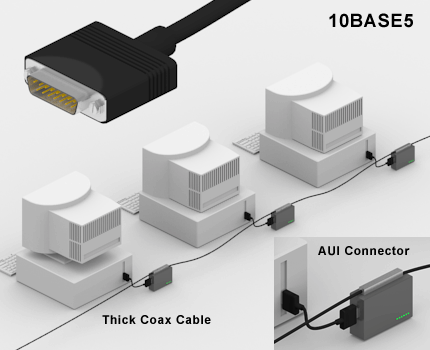
\includegraphics[width=0.6\linewidth]{Figures//06/thicknet.png}
    \caption{Rappresentazione di rete Thicknet. Fonte: \href{https://www.computerlanguage.com/results.php?definition=thick+Ethernet}{ComputerLanguage.com}}
    \label{fig:06thicknet}
\end{figure}
\begin{figure} [ht]
    \centering
    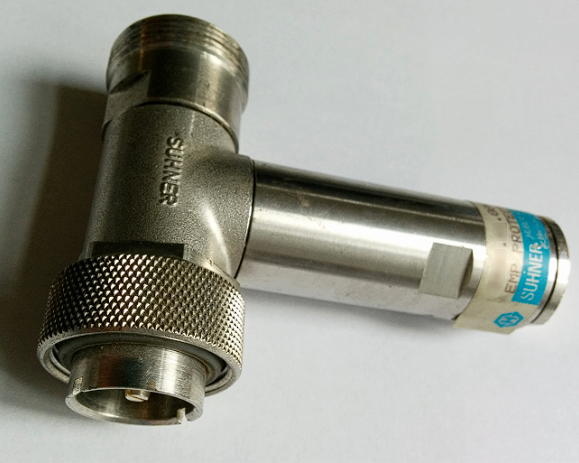
\includegraphics[width=0.5\linewidth]{Figures/06/Tconn.png}
    \caption{Connettore T per reti Thinnet. All'estremità ``lunga'' viene collegato il terminale, a quelle corte rispettivamente l'input e il resto del ring (o un Terminatore, tipo un tappo a impedenza $50\Omega$ di tipo BNC come le altre estremità dei coassiali)}
    \label{fig:06T}
\end{figure}

\noindent Doppino telefonico:\index{doppino}
\begin{itemize}
    \item non ci si collega più ad un bus comune ma a degli Switch;
    \item connettori BNC sostituiti da connettori RJ45;
    \item max distanza 100m.
\end{itemize}

\noindent La disposizione dei fili all'interno del connettore RJ45\index{RJ45} determina che tipo di collegamento si sta creando (schema T568-A, T568-B, in Fig. \ref{fig:06RJ45}):
\begin{itemize}
    \item se si realizza un cavo con connettori uguali a entrambe le estremità (quindi A-A o B-B), il cavo sarà di tipo straight-through;
    \item se si configurano connettori diversi (A-B, B-A), il cavo esce di tipo cross-over;
\end{itemize}

\begin{figure} [ht]
    \centering
    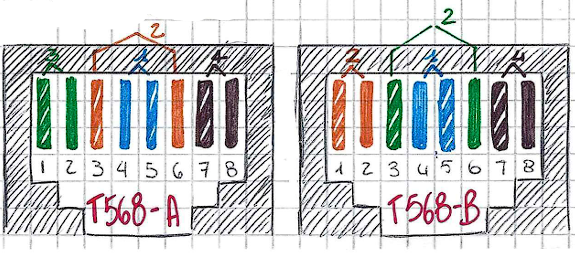
\includegraphics[width=0.75\linewidth]{Figures//06/rj45ab.png}
    \caption{Schema delle binature T568-A e T568-B.}
    \label{fig:06RJ45}
\end{figure}

\noindent Doppini:\index{doppino}\index{T568-A, T568-B}
\begin{itemize}
    \item UTP: doppino non-schermato (Unshielded Twisted Pair);\index{UTP}
    \item FTP: doppino schermato con foglio di alluminio + collegamento a massa (Foiled Twisted Pair);
    \item STP: doppino con schermo locale (Shielded Twisted Pair);
    \item S-UTP / S-FTP: doppino con schermo locale e foglio di alluminio.
\end{itemize}


\newpage
\noindent Categorie:\index{doppino!CAT}
\begin{itemize}
    \item [CAT 1]: solo per segnali vocali (telefonia);
    \item [CAT 2]: max vel. 4Mbps;
    \item [CAT 3]: max vel. 10Mbps;
    \item [CAT 4]: max vel. 16Mbps;
    \item [CAT 5]: max vel. 100Mbps con banda passante 100MHz;
    \item [CAT 5e]: max vel. fino a 1Gbps;
    \item [CAT 6]: max vel. fino a 10Gbps, banda passante fino a 250MHz;
    \item [CAT 7]: non riconosciuto da EIA/TIA.
\end{itemize}
\noindent N.B.: queste note sono state redatte inizialmente nel 2021, quindi non sono da escludere nuovi sviluppi di standard del doppino. Per preservare l'intreccio dei cavi interni, le norme di installazione vogliono che non si eserciti una forza superiore a $11,3$ Kg (insomma, non tirare i cavi così forte).\\

\addcontentsline{toc}{subsection}{Fibra Ottica}
\subsection*{Fibra Ottica}
\index{fibra ottica}
\begin{figure} [ht]
    \centering
    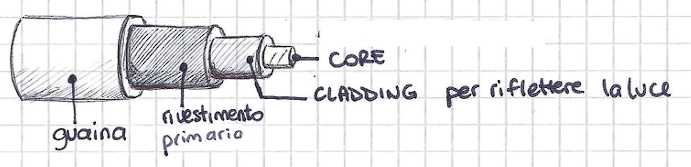
\includegraphics[width=0.75\linewidth]{Figures//06/of.png}
    \caption{Schema della struttura interna di un cavo di fibra ottica.}
    \label{fig:06OF}
\end{figure}\index{fibra ottica!cavo}
\begin{itemize}
    \item la fibra ottica, al contrario del coassiale e del doppino (che hanno bisogno di tutte quelle schermature) è immune alle interferenze;
    \item può essere:
    \begin{itemize}
        \item monomodale;
        \item multimodale (trasmette luce su più frequenze);
    \end{itemize}
    \item  tipo di connettore: ST (Straight Tip), o più spesso SC (Standard Connector).
\end{itemize}

\addcontentsline{toc}{section}{Estensione di una LAN}
\section*{Estensione di una LAN}\index{LAN!estensione}
\noindent Perché estendere una LAN?
\begin{itemize}
    \item unificare LAN costruite in momenti diversi;
    \item unificare LAN situate in diversi edifici; 
    \item distribuire carichi di traffico elevati;
    \item aumentare la distanza copribile;
    \item aumentare l'affidabilità;
    \item aumentare la sicurezza.
\end{itemize}
\noindent Ci sono naturalmente delle limitazioni dovute a protocolli di accesso e al decadimento del segnale - non si può espandere all'infinito, insomma.\\
\noindent Come estendere una LAN?
\begin{itemize}
    \item con dei Repeater\index{repeater} (Layer 1 device): come un buffer di segnale;
    \item  con dei Bridge\index{bridge} (Layer 2 device): leggono l'intestazione dei frame e inoltrano in base al contenuto che leggono. Non propagano collisioni. Sono adattivi, ovvero si configurano a mano a mano che ricevono informazioni sulla rete (credo facciano similmente agli switch). È possibile collegare con un bridge anche reti con tecnologie diverse, ad esempio Ethernet con Token Ring.
\end{itemize}

\begin{figure} [ht]
    \centering
    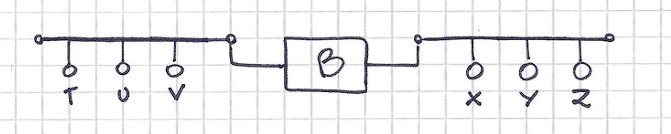
\includegraphics[width=0.75\linewidth]{Figures//06/bridge.png}
    \caption{Bridge B collega due LAN di host TUV e XYZ.}
    \label{fig:06bridge}
\end{figure}

\begin{itemize}
    \item Transparent Bridge: se X deve comunicare con Z nell'esempio in Fig. \ref{fig:06bridge}, la prima volta il frame viene inoltrato lungo TUTTA la rete, ma al ritorno il bridge avrà già appreso che X e Z sono nella stessa porzione di rete, quindi eviterà di inoltrarlo alla parte con TUV. (Backward Learning)
    \item Source Node Bridge: i bridge non mantengono queste informazioni di routing, ma sono capaci di selezionare il percorso ottimale tra due punti.
\end{itemize}
\noindent Ciclo di Bridge: dovuto a flooding, alcuni frame rimangono in circolo a lungo senza raggiungere una destinazione. Soluzione: Distributed Spanning Tree Protocol (STP), serve per far comunicare i bridge, in breve.\\

\addcontentsline{toc}{subsection}{Fault Tolerance}
\subsection*{Fault Tolerance}\index{fault tolerance}
\begin{figure}
    \centering
    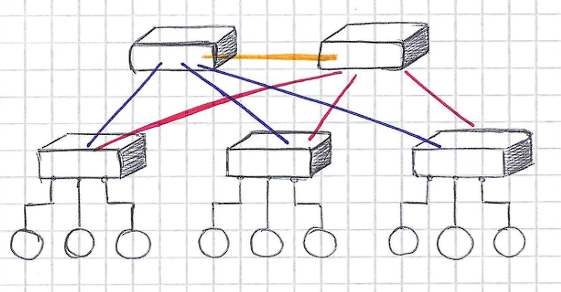
\includegraphics[width=0.75\linewidth]{Figures/06/ft.png}
    \caption{Centro Stella Ridondato, meccanismo di fault tolerance}
    \label{fig:06csr}
\end{figure}
\noindent Si costruisce una rete con doppi concentratori (Fig. \ref{fig:06csr}), in modo tale che se uno dovesse smettere di funzionare, l'altro terrebbe comunque in normale funzione il servizio. Aggiungere dispositivi ``di scorta'' prende il nome di Ridondanza.\\
\noindent Gli switch possono essere stackati (ad esempio, se ne può creare uno a 96 porte impilandone 2 da 48). Gli switch si possono gestire con CLI o GUI, accessibili via cavo o remote shell.\\ 
\noindent La tecnologia VLAN (Virtual LAN)\index{LAN!virtuale(VLAN)} serve a dividere virtualmente un solo switch in più LAN.\\
\noindent Reti Commutate (con Switch) $\approx$ come un mega bridge, in un certo senso. Lavorano in 3 modalità:\index{rete!commutata}
\begin{itemize}
    \item Cut-Through: lo switch legge il MAC, inoltra dove deve, fine.
    \item Store \& Forward: Legge il MAC, immagazzina tutto il messaggio e ne controlla i CRC, inoltra se tutto ok;
    \item Fragment Free: una via di mezzo, legge solo i primi 64 Byte del frame e fa controlli solo su quel prefisso. Se tutto ok, inoltra. (tant'è che, a differenza del header IP, nello header MAC viene prima il campo Destinazione poi Sorgente)
\end{itemize}